%% This is an example first chapter.  You should put chapter/appendix that you
%% write into a separate file, and add a line \include{yourfilename} to
%% main.tex, where `yourfilename.tex' is the name of the chapter/appendix file.
%% You can process specific files by typing their names in at the 
%% \files=
%% prompt when you run the file main.tex through LaTeX.
\chapter{Data Analysis}

\section{Analysis Tools}

In this thesis, the analysis tools we use is based on Macbook computers, and CMS high computing, linux shell script, C++ programing language, and ROOT analysis package for high energy physics experiments. The machine performing the analysis includes CERN lxplus, MIT Tier-2 submit, Data file are saved as ROOT files format. Data samples are processed with crab CERN lxplus and MIT submit condor job submission with parallel computing framework. The core software for the data process and analysis is the CMS software (CMSSW\_10\_3\_4). The codes for the analysis software is documented on github and gitlab. Throughout the analysis, we use Poison statistics to interpret the statistical uncertainties of the data. In the limit of high statistics, it is approximately equivalent to Gaussian Statistics. In the limit of low statistics, it is different from Gaussian Statistics. These tools are crucial for me to finish the analysis and present the results.

\section{Analysis Strategies}

\subsection{Physics Goals}

The exclusive productions of b hadrons in different collision systems are necessary to study beauty energy loss and hadronization mechanisms. In this thesis, we propose to fully reconstruct $B^0_s$ and $B^+$ mesons in pp and PbPb collisions at $\sqrt{s_{NN}} = $ 5.02 TeV with the CMS experiment. We aim at measuring precisely their cross section, yield ratios, and nuclear modification factor of fully reconstructed $B^0_s$ and $B^+$ mesons via the decay channels of  to investigate beauty quark production and hadronization in vacuum and QGP. We hope to have a conclusive measurement of $B^0_s/B^+$ ratio to pinpoint the effect of strangeness enhancement in QGP on beauty hadronization and test theoretical model calculations \cite{StrangetoLight} with both fragmentation \cite{} and quark coalescence \cite{} mechanisms. Therefore, we would like to present our experimental measure over a width range of $p_T$ and centrality. We are particularly interested in the very low $p_T$ region where the slow moving beauty quark will pick up the nearby light quarks in the QGP while such mechanism is not expected to occur in the vacuum \cite{}. The $R_{AA}$ down to low $p_T$ will constrain understand beauty quark energy mechanism in the QGP medium. These will studies will be crucial for us to understand beauty quark diffusion coefficient and probe the inner workings of QGP in order to provide insights with the one of the open question in high energy nuclear physics.

\subsection{General Workflow}

Figure \ref{BsBPWorkFlow} shows workflow we designed to fully reconstructed $B^0_s$ and $B^+$ mesons from final state particles via the exclusive decay modes. The $B^0_s$ is fully reconstructed from the decay channel of $B^0_s \rightarrow J/\psi \phi \rightarrow \mu^+\mu^- K^+K^-$, which has a fragmentation fraction of $f(b\rightarrow B_s^0) =$ 0.103 and a decay branching fraction $BR(B^0_s \rightarrow J/\psi \phi \rightarrow \mu^+\mu^- K^+K^-) = 1.35 \times 10^{-5}$ $B^+ \rightarrow J/\psi K^+\rightarrow \mu^+\mu^- K^+$ with the CMS detector. 


\begin{figure}[hbtp]
\begin{center}
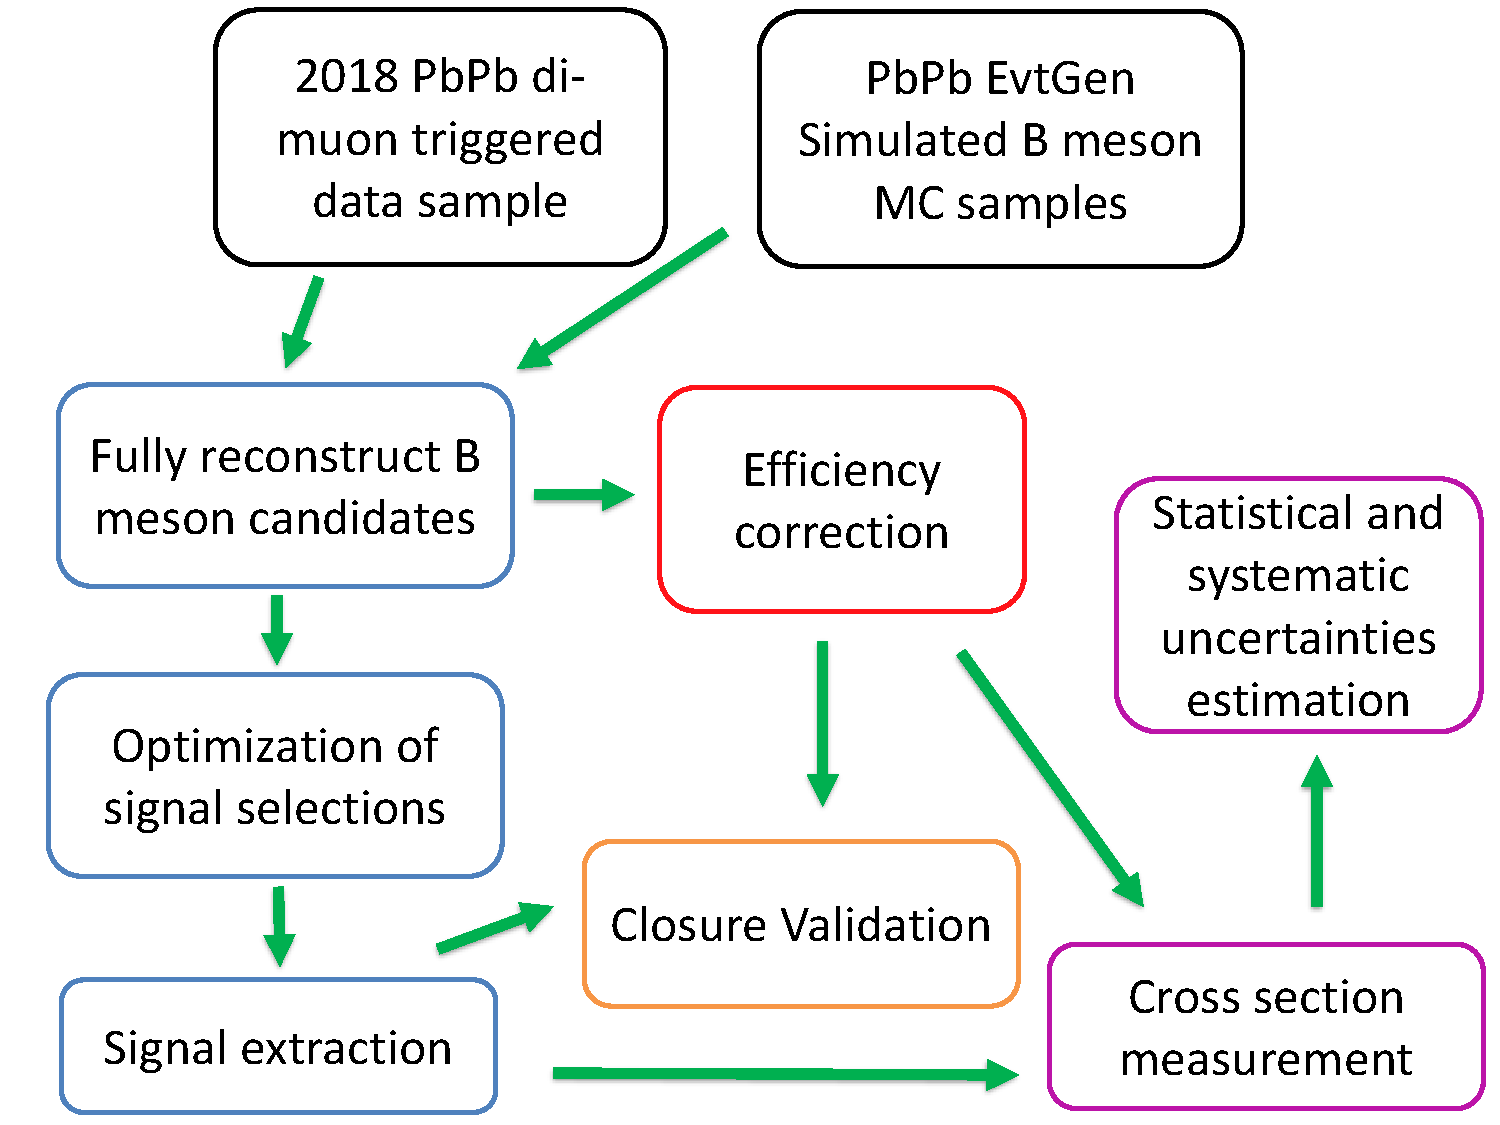
\includegraphics[width=0.65\textwidth]{Figures/Chapter4/BsBPWorkFlow.pdf}
\caption{The block diagram of the workflow with major steps for both B-meson cross section measurement is shown above.}
\label{BsBPWorkFlow}
\end{center}
\end{figure} 

Figure \ref{BsBPRECO} shows pictorially the decay topology of fully reconstructed B meson and our reconstruction strategies are

\begin{figure}[hbtp]
\begin{center}
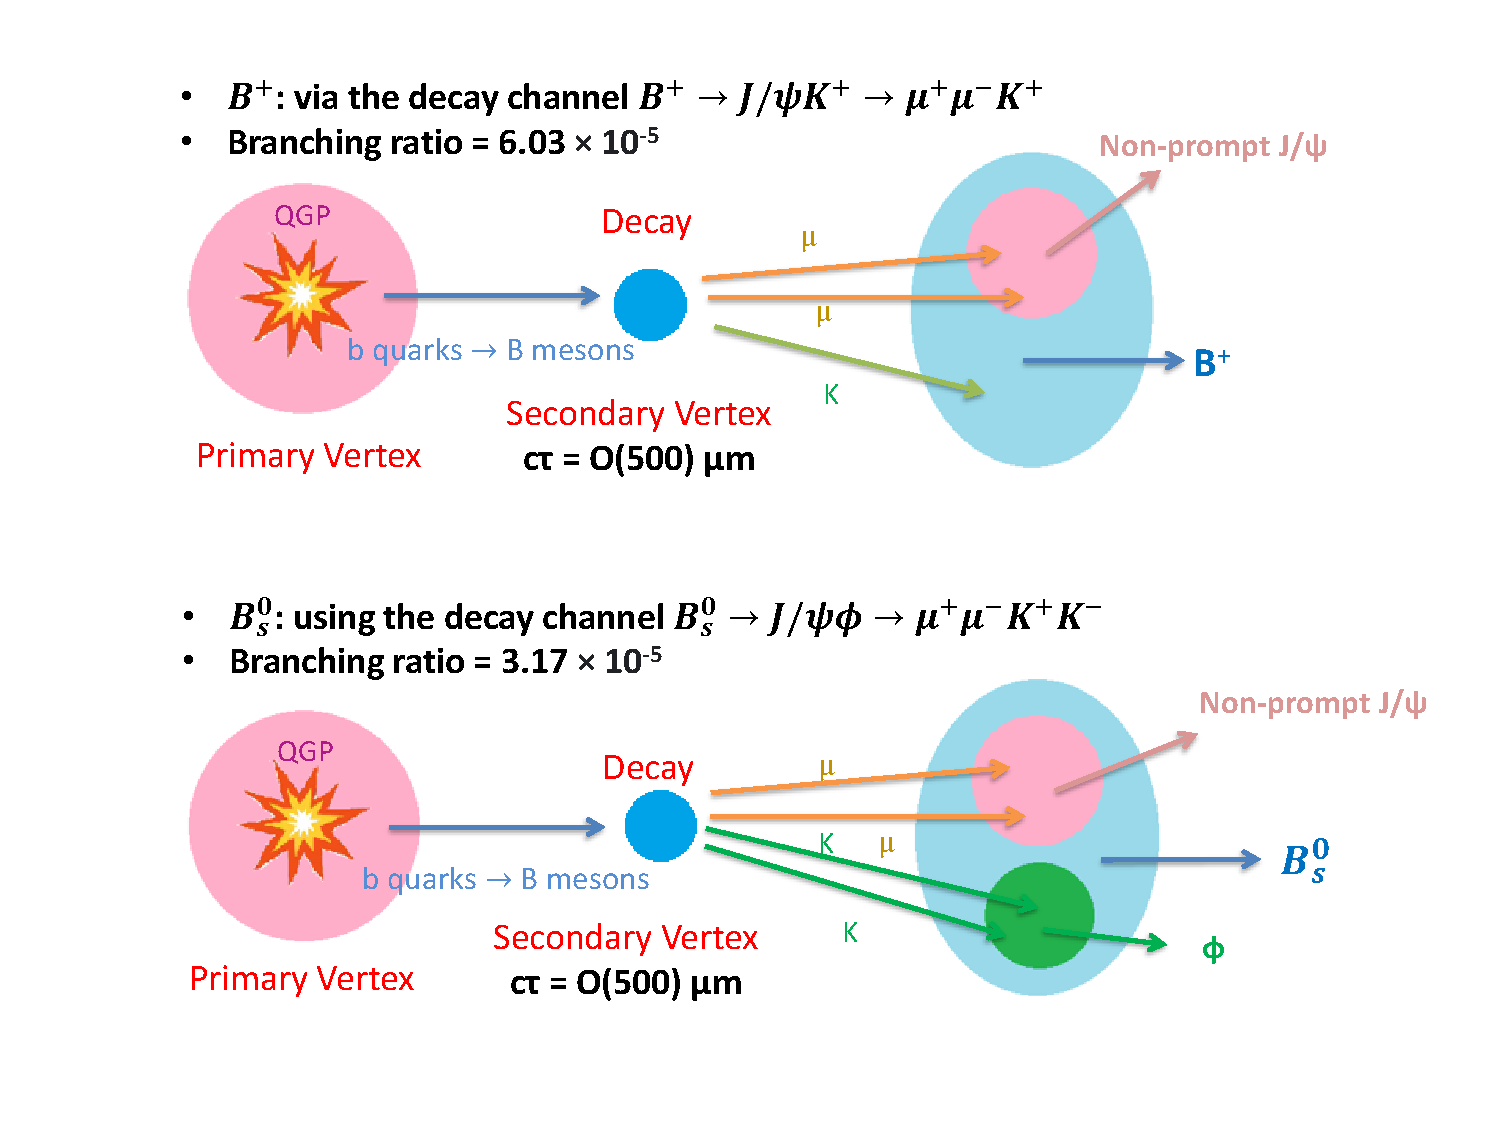
\includegraphics[width=0.86\textwidth]{Figures/Chapter4/BsBPRECO.pdf}
\caption{The strategies to fully reconstruct $B^0_s$ and $B^+$ in the selected exclusive decay modes are shown above.}
\label{BsBPRECO}
\end{center}
\end{figure} 


\subsection{Technical Challenges}

Despite the excellent muon, tracking, vertexing capabilities of the CMS detector, there are still many challenges for the analysis. Below is a list of challenges in the B-meson analysis 

\begin{itemize}
\item The small B meson decay branching ratio, which on in the order of 10$^{-5}$, and limited luminosity of the sample: $S \downarrow$ 
\item Huge combinatorial background without hadron particle identification, particularly in PbPb collisions and at low $p_T$:  $B \uparrow$ 
\item Low muon acceptance of at very low $p_T$: $S \downarrow$ 
\item High fake track rate with low tracking efficiency at very low $p_T$: $B \uparrow$ 
\end{itemize}

Here, $S$ stands for signal and $B$ stands for background. These factors will all lower the signal-to-background ratio, which makes challenging to fully reconstruct B mesons, particularly at very low $p_T$. In this thesis, to reduce the signal to background ratio and the systematic uncertainties, we will employ a novel approaching machine learning with multivariate analysis and the elaborated single particle efficiency correction method to perform the measurements.


\section{Analysis Samples}

\subsection{Dimuon Triggered Datasets}

In this part of the thesis, I focus on the studying beauty production and hadronization in QGP. Therefore, this analysis is performed using the 2018 PbPb data at $\sqrt{s_{NN}}$=5.02 TeV, which has an integrated luminosity of 1.7 $nb^{-1}$. 
The analysis uses the dimuon primary datasets (\textit{DoubleMu} PD). The full name of the used datasets and their corresponding luminosity can be found in Table~\ref{tab:lumi}.

\begin{table}[htb]
\begin{center}
\caption{List of PbPb HLT datasets and triggers with the corresponding integrated luminosities used in the analysis.}
\label{tab:lumi}
 \tiny
 \begin{tabular}{ l | l | l | l | }
 System& Primary dataset & Trigger & Luminosity\\
  \hline\hline 
PbPb & \verb#/HIDoubleMuonPsiPeri/HIRun2018A-04Apr2019-v1/AOD# & \verb# HLT_HIL3Mu0NHitQ10_L2Mu0_MAXdR3p5_M1to5_v1 # & 522 $nb^{-1}$\\
  PbPb & \verb#/HIDoubleMuon/HIRun2018A-04Apr2019-v1/AOD # & \verb# HLT_HIL3Mu0NHitQ10_L2Mu0_MAXdR3p5_M1to5_v1 # & 1124 $nb^{-1}$ \\
  \hline
  PbPb & Combined All & & 1.657 ($\sim$ 1.7) $nb^{-1}$ \\
 \end{tabular}
\end{center}
\end{table}

The details of the dimuon trigger selection to collect the data sample is explained in 2.2.5. In addition, an Muon JSON to select good luminosity sections in the PbPb dataset is applied. Both $B^0_s$ and $B^+$ data come from this sample. However, in the later stage, the B meson candidates are saved in different channels based on the reconstruction.

\subsection{Monte Carlo Simulations Samples}

Dedicated PbPb $B^0_s$ and $B^+$ samples are generated in order to estimate the acceptance and selection efficiencies, to study the background components, and to evaluate systematic uncertainties. {\sc PYTHIA8} Tune CUETPM8~\cite{PYTHIAFrag,PYTHIA2}, set to generate inclusive (all quark/antiquark, as well as gluon initiated) QCD processes, was used to generate at 5.02 TeV the signal. Several preselections at the generation steps are applied in order to optimize the generation process and conserve resources.

For $B^0_s$, only signal events were kept with at least one $B^0_s$ (forced to decay through the channel $B^0_s \rightarrow J/\psi \phi \rightarrow \mu^+\mu^-K^+K^-$ by means of the {\sc evtgen} package~\cite{EvtGen}), with $p_{T}>$ 5.0 GeV/c, and $|\eta|<$ 2.4. In addition, the $J/\psi$ and $\phi$ meson, are forced to decay in the two muons and two kaons respectively. Final state radiations are generated using {\sc photos}~\cite{PHOTOS}. The selected signal B mesons {\sc PYTHIA8} events were embedded into a PbPb background simulated with the {\sc HYDJET}  (version 1.8, tune ``Drum'' for the prompt and non-prompt $J/\psi$ MC and tune "Cymbal5Ev8" for the $B^0_s$ signal MC)~\cite{HYDJET} event generator.

For $B^+$, similar requirements for MC generation are applied except a different decay channel $B^0_s \rightarrow J/\psi K^+ \rightarrow \mu^+\mu^-K^+$ is used.

For $B^0_s$ and $B^+$, around fifty thousand events were generated in 5 $\hat{p}_{T}$ bins, with boundaries of $\hat{p}_{T} >$ 0, 5, 15, 30, 50, in both signal only, and embedded samples. The high $\hat{p}_{T}$ selections are used to enrich the high $p_T$ B meson statistics in order to perform efficiency correction. 

We should note that in there are two components in the MC sample. The truth information about the particles generated in the simulation, which is call generated (GEN), and the reconstructed one smeared according to the CMS detector effects, which is called reconstructed (RECO). Due to the nature of MC generation, we will need to reweigh on MC in order to model the data.


\subsection{$\hat{p}_{T}$ Reweighing}


As we mention above, different $\hat{p}_{T}$ cut is applied to generate the MC samples. When merging the samplings, a  $\hat{p}_{T}$ weight based on beauty production cross section is required to apply to the MC in order to obtain a smooth distribution that can model the real data. Figure \ref{GENPTDIS} shows the generated $p_T$ ($Gp_T$) distribution of $J/\psi$, $B^+$ , and $B^0_s$ before and after applying the $\hat{p}_{T}$ weight:


\begin{figure}[h]
\begin{center}
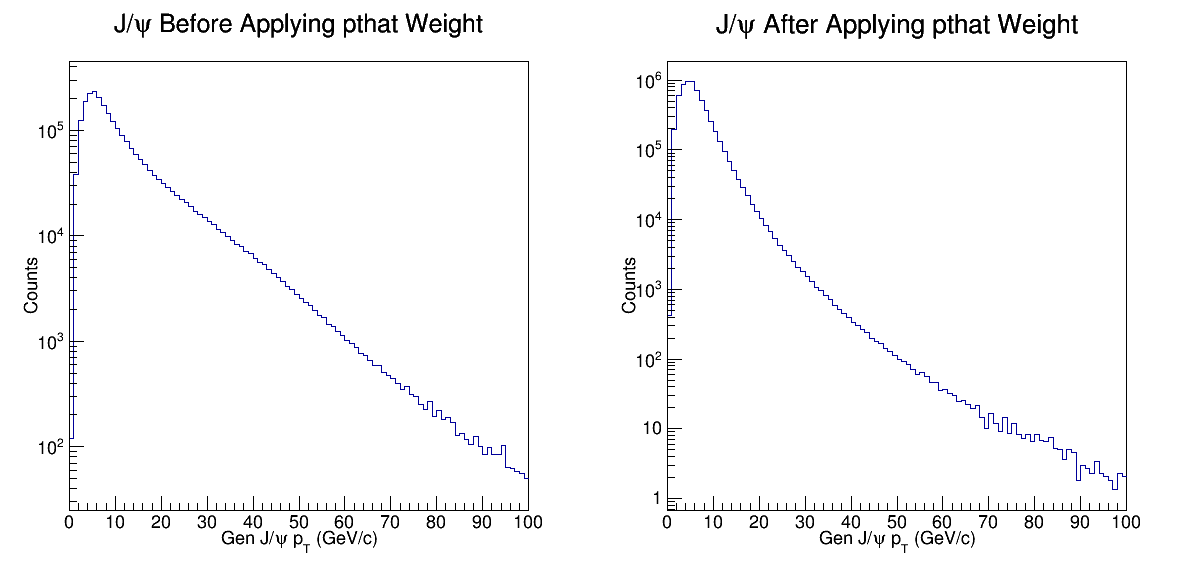
\includegraphics[width= 0.90\textwidth]{Figures/Chapter4/JPsiGenpT.png}
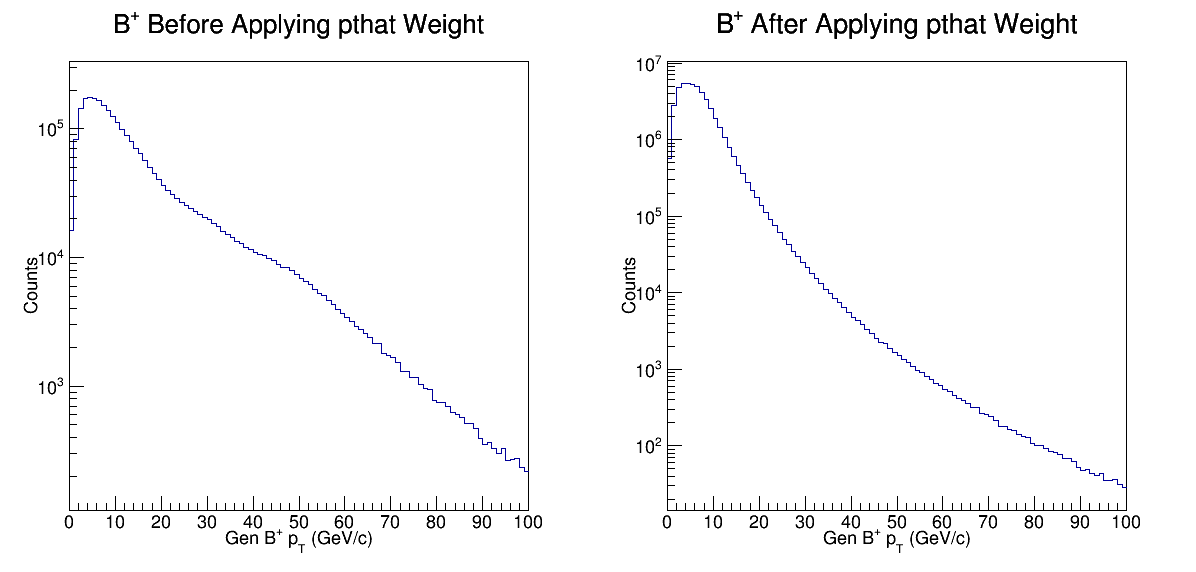
\includegraphics[width= 0.90\textwidth]{Figures/Chapter4/BPlusGenpT.png}
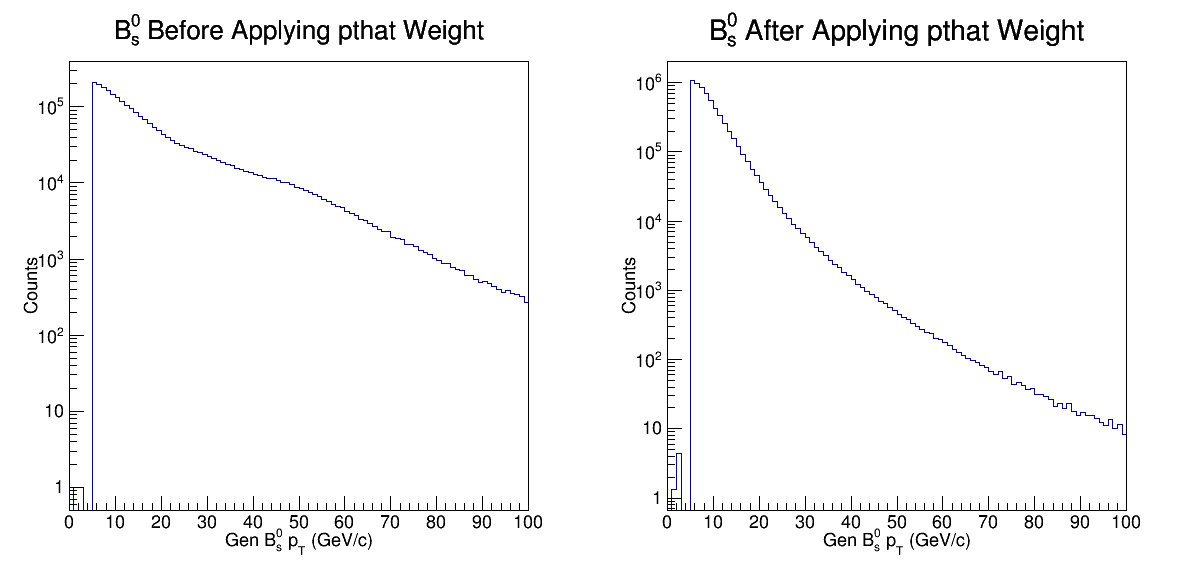
\includegraphics[width= 0.90\textwidth]{Figures/Chapter4/BsGenpT.png}
\caption{ $J/\psi$ generated $p_{T}$ distribution before (upper left) and after (upper right) $\hat p_{T}$ reweighing, $B^+$ generated $p_{T}$ distribution before (middle left) and after (middle right) $\hat p_{T}$ reweighing, and $B_s^0$ generated $Gp_{T}$ distribution before (lower left) and after (lower right) $\hat p_{T}$ reweighing are shown above.}
\label{GENPTDIS}
\end{center}
\end{figure}


\subsection{RECO B-meson ${p}_{T}$ Reweighing}

Then, we also check if this smooth $Gp_T$ shape in fact correspond to a good agreement between the data and MC in the RECO side. Therefore, we take the ratio of the normalized data raw yield to the normalized MC raw yield and perform a variety of functions to fit the distribution. In our studies, we use Linear ($y = p_0 + p_1 x$), Quadratic ($y = p_0 + p_1 x + p_2 x^2$), Linear + Inverse  ($y = p_1 x + \frac{p_2}{x}$), Linear + Square Root ($y = p_0 + p_1 x + p_2 \sqrt{x}$), Linear + Log ($y = p_0 + p_1 x + p_2 \log{x}$). The data vs MC raw yield shape and our fitting results on spectra ratio are show as follows \ref{BsBptWeight} and  \ref{BPBptWeight} for $B^0_s$ and $B^+$ respectfully 



\begin{figure}[h]
\begin{center}
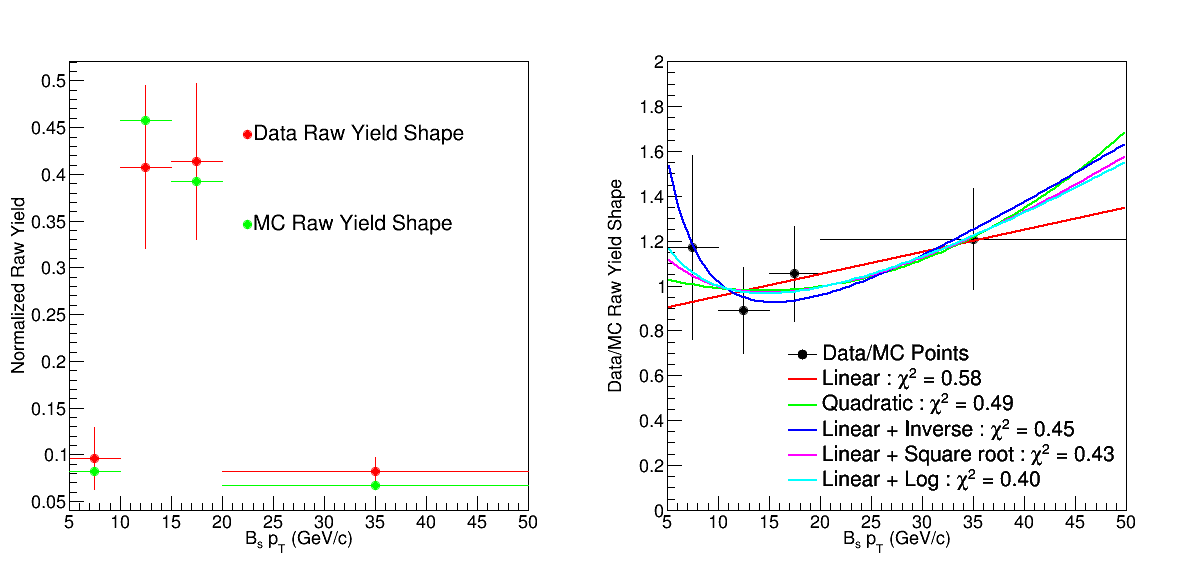
\includegraphics[width= 0.97\textwidth]{Figures/Chapter4/BsBptDataMC.png}
%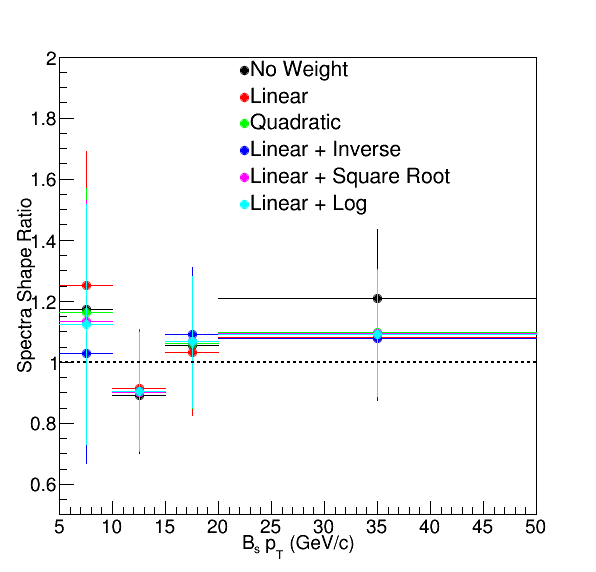
\includegraphics[width= 0.55\textwidth]{Figures/Chapter4/BsBptDataMCAfter.png}
%\caption{ $B^0_s$ $p_T$ normalized raw yields obtained in PbPb MC and Data are shown above on the top left panel. The data/MC ratio and different fitting functions: Linear (Red), Quadratic(Green), Linear + Inverse (Blue), Linear + Square Root (Purple), and Linear + Log (Cyan) and their $\chi^2$ are shown above on the top right panel. The bottom plots are the data/MC reweighed yields with different functions from the fit on the top right panel. We can see that they all get closer to unity compared unweighted MC. The Linear + Log (Cyan) line, which has the smallest $\chi^2$ and is closest to unity after applying the weight to the MC. Hence, Linear + Log function is use as nominal for our $B^0_s$ $p_{T}$ reweighing. All other fitting function are used as reference to calculate the $p_T$ shape systematic uncertainties.}
\caption{ $B^0_s$ $p_T$ normalized raw yields obtained in PbPb MC and Data are shown above on the top left panel. The data/MC ratio and different fitting functions: Linear (Red), Quadratic(Green), Linear + Inverse (Blue), Linear + Square Root (Purple), and Linear + Log (Cyan) and their $\chi^2$ are shown above on the top right panel. The bottom plots are the data/MC reweighed yields with different functions from the fit on the top right panel.}
\label{BsBptWeight}
\end{center}
\end{figure}

\begin{figure}[h]
\begin{center}
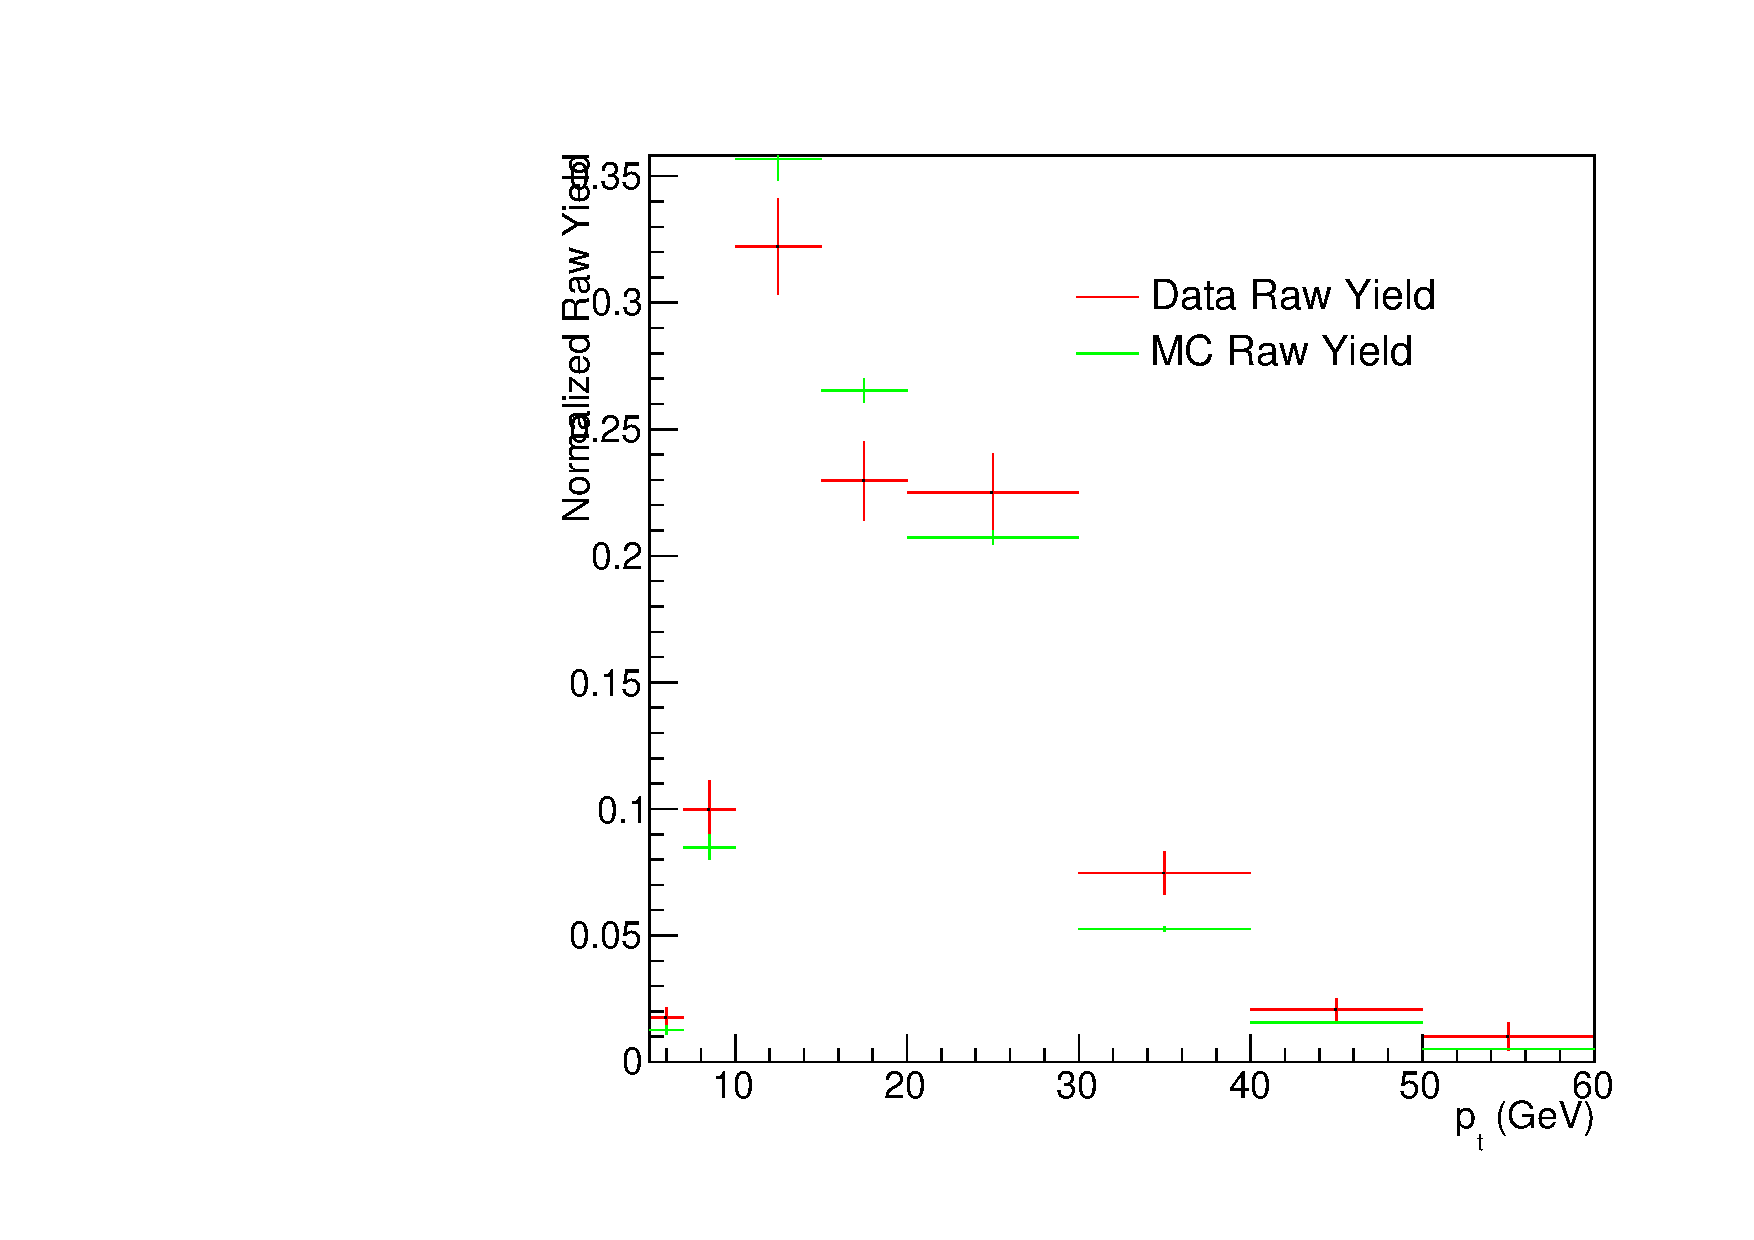
\includegraphics[width= 0.48\textwidth]{Figures/Chapter4/BPBptDataMC1.pdf}
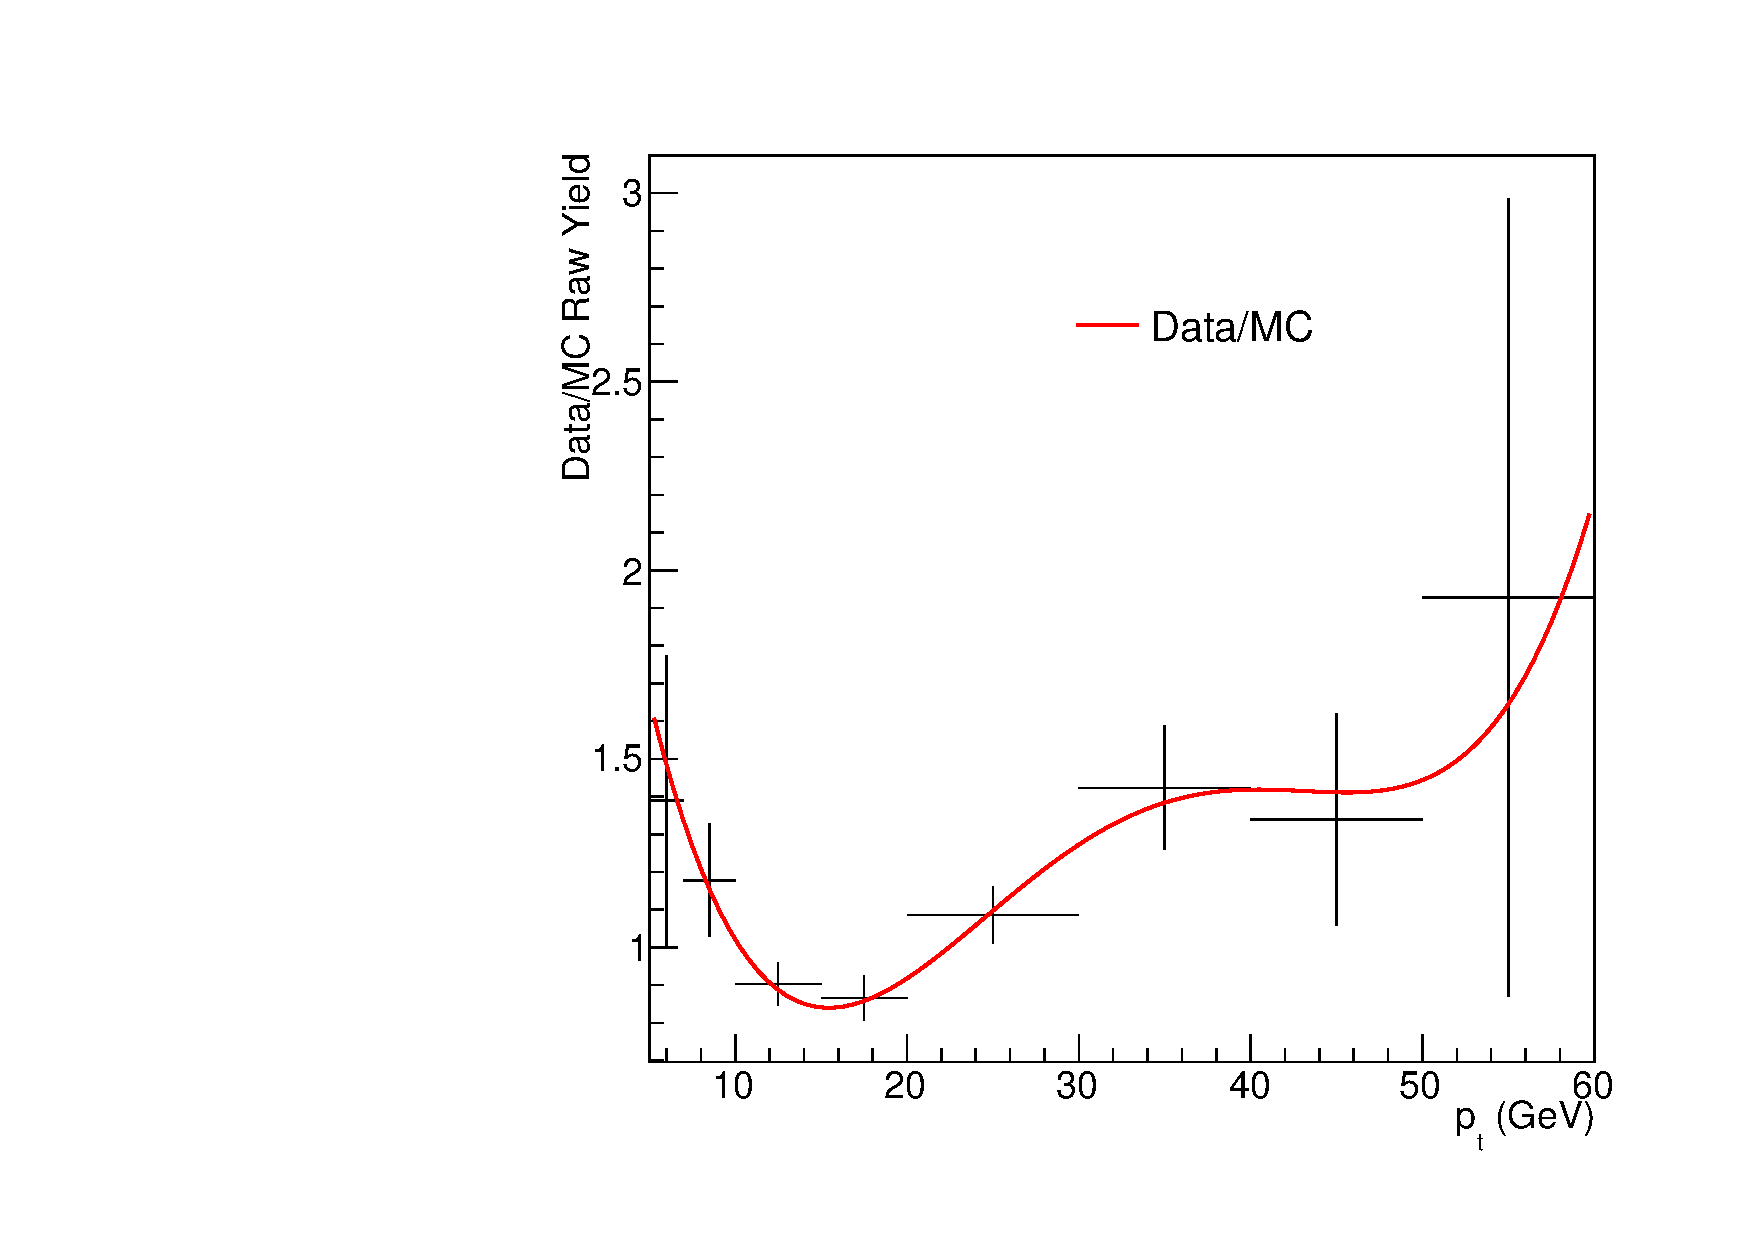
\includegraphics[width= 0.48\textwidth]{Figures/Chapter4/BPBptDataMC2.pdf}
\caption{The normalized $B^+$ raw yield in MC (green) and Data (red) as a function RECO $B^+$ $p_T$ (left) and the fourth order polynomial fits to their ratio (right) are shown above.}
\label{BPBptWeight}
\end{center}
\end{figure}


\subsection{Centrality Reweighing}

Because the MC simulations employ PYTHIA embedded into a PbPb background simulated, they do not model the centrality of nucleus-nucleus collision well. Therefore, the MC simulations are also reweighed in order to match the centrality distribution in data. In the middle panel of Figure \ref{CentComp}, the centrality distribution of the MC simulation (red) is compared to the one in data (blue), before the re-weighting. Each unit (hiBin) on the x-axis represents 0.5\% centrality. The number of binary collisions $N_{coll}$ was used as the weight to scale the MC centrality, and the distribution presented in the right panel of Figure 4 was obtained. 

\begin{figure}[hbtp]
\begin{center}
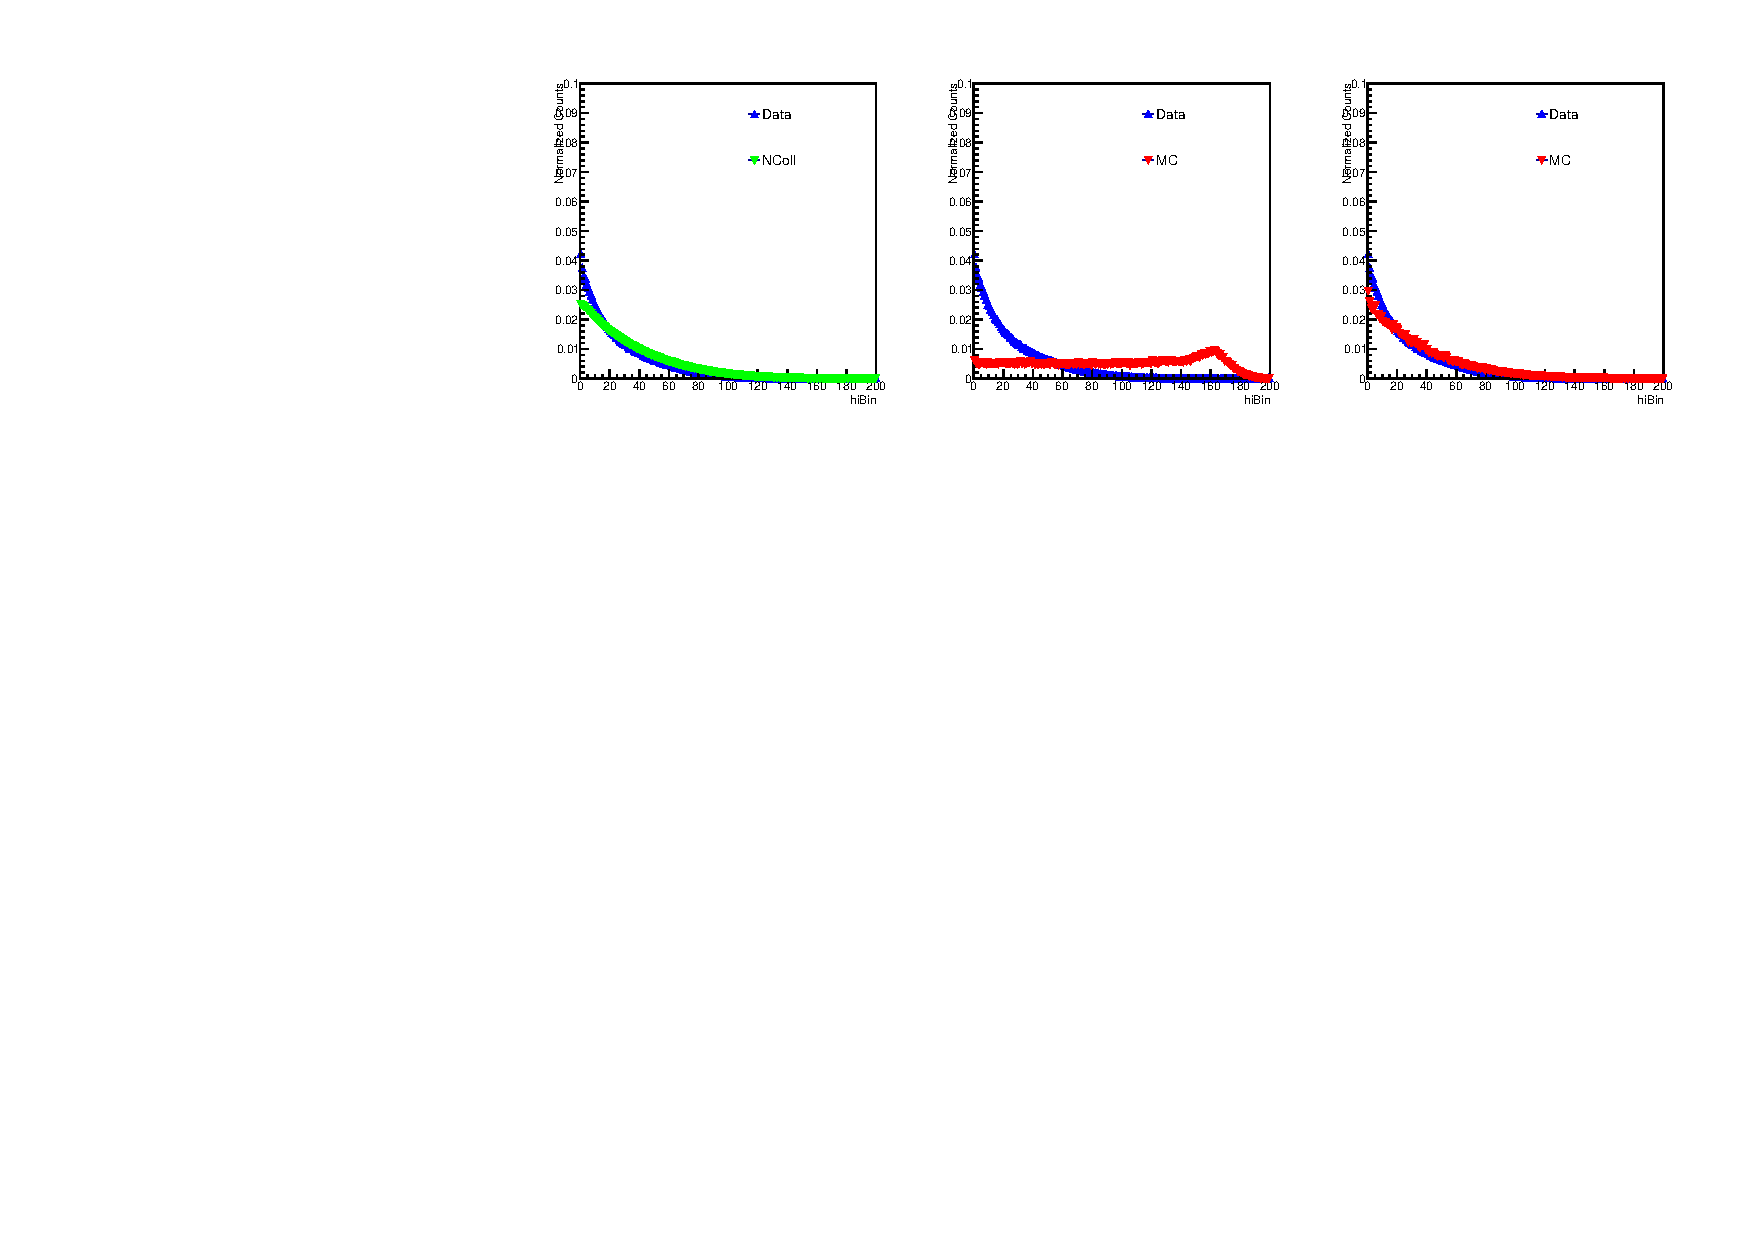
\includegraphics[width=1.10\textwidth]{Figures/Chapter4/CentralityWeight.pdf}
\caption{The comparison between $N_{coll}$ and Data vs hiBin (left), centrality distribution of MC (red) and data (blue) in PbPb collisions in the centrality interval 0-100\% without $N_{coll}$ weight (middle), and with $N_{coll}$ weight (right) are shown above.}
\label{CentComp}
\end{center}
\end{figure} 


A better centrality agreement between the data and the MC is seen after the reweighing process. 

\subsection{PV$_{z}$ Reweighing}


In addition to above pt shape and centrality reweighing, there must be a primary vertex $z$ position (PV$_{z}$) reweighing due to incorrect modeling of the primary vertex location and resolution in the MC simulation. In fact, it is known that the MB samples use for embedding for PbPb signal MC samples (with Cymbal5Ev8 tune) has a PV$_{z}$ offset. Also, the offsets between data and MC in the X and Y directions are observed in the 2018 PbPb collisions. To remedy this, a Gaussian fit is applied to both the data and MC PV$_{z}$ distributions, as showed in Fig.~\ref{PVZPlot}. The black markers represent the distribution points for MC (left), and data (right), while the red line represents the fit result. Then, the ratio between the two fit results is taken as the weighting function. The result after this weighting can be found in Fig. \ref{PVZPlot} But we should note that this analysis is not sensitive to the absolute value of the PV position because the reconstruction of the B-meson rely only on the relative distance between PV and B-meson reconstructed vertex which will be presented in the later sections.

\begin{figure}
\begin{center}
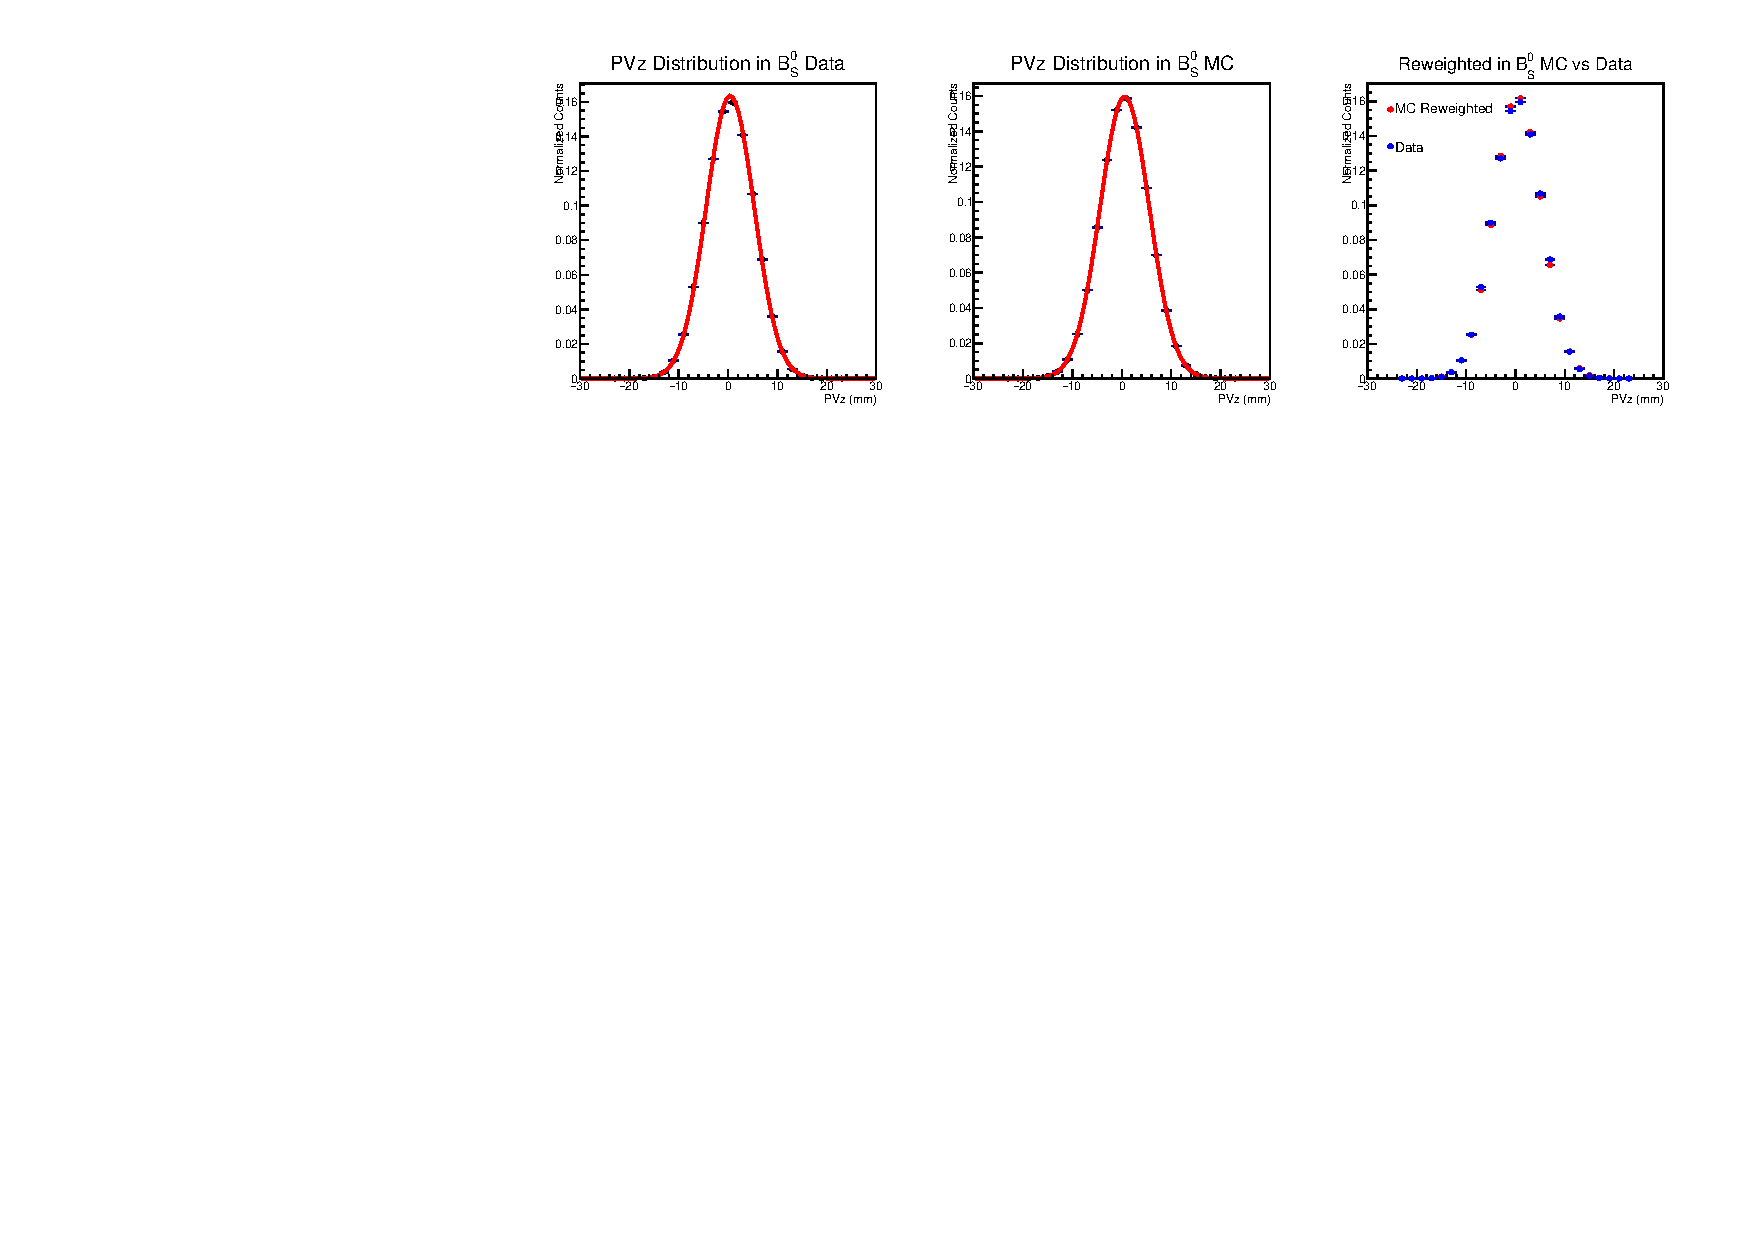
\includegraphics[width= 1.10\textwidth]{Figures/Chapter4/PVzWeightPbPb.pdf}
\caption{Primary vertex z position (PV$_{z}$) distribution, fitted with a gaussian function in PbPb MC simulations (left), in PbPb data (middle), PV$_{z}$ reweighed MC to data with ratio of data-to-MC Gaussian Fits (right) are shown above. The PV$_z$ distributions are well described by the Gaussian function and reweighing reduces the MC-data discrepancy.}
\label{PVZPlot}
\end{center}
\end{figure}

A almost perfect MC-data agreement after PV$_{z}$ reweighed is observed above. After these standard reweighing procedures, the residue disagreement between MC and data will be considered as a source of systematic uncertainties.


\clearpage

\section{Global Event Observables} 

The global event observables characterize general conditions of heavy-ion collision. In this analysis, we decide to use another set of quantities including total number of MB events to represent the luminosity and average number of participants $N_{parts}$ to represent centrality. In addition, to compare with $pp$ collisions, we also need to scale the cross section in PbPb according to . Therefore, we will determine the all the global event observable including total number of minimum bias events ($N_{MB}$), centrality, number of participant nucleons $N_{part}$, number of binary collisions $N_{coll}$, and nuclear overlapping function $T_{AA}$ in dimuon PbPb dataset in the follow subsections.

\subsection{Total Number of Events}

As seen in Table \ref{tab:lumi}, the nominal luminosity of the dimuon PbPb dataset 1.7 $nb^{-1}$. However, this nominal luminosity has large uncertainties and should be used in the analysis to measure the cross section. As mentioned previous in Chapter 2.2, the dimuon trigger, based on the MB trigger, will not save events that does not pass trigger selections. Hence, we can use the events of 1 PD MB datasets (PD0) via the follow formula to determine the actual number of MB events corresponding to the dimuon PbPb datasets: 


\begin{equation}
N_{MB} = \frac{N^{\mu\mu json}_{MB}}{\mathcal{L}_{MB trigger}^{\mu json}} \mathcal{L}_{\mu\mu trigger}^{\mu\mu json}
\end{equation}

The definition of the variables in the formula are as follows:


\textbf{$N_{MB}$:} The number of minimum bias events in dimuon PD with muon json.

\textbf{$N^{\mu json}_{MB}$:} The number of event of all MB PDs with muon json. 

\textbf{$\mathcal{L}^{\mu json}_{MB}$:} The luminosity of all MB PDs with muon json.

\textbf{$\mathcal{L}_{\mu\mu trigger}^{\mu\mu json}$:} The luminosity of dimuon PD with muon json.

\iffalse 

To obtain the total number of minimum bias $N_{MB}$, first we process one PD (PD5) minimum bias events and count the total number of events for centrality at 0 - 90\% to obtain $N^{\mu\mu json}_{MB}$. Then, we run the brilcal for MB PD5 and sum the luminosity of HLT MB triggers: 

Trigger 1: ``HLT\_HIMinimumBias\_part0\_v1" 
 
Trigger 2: ``HLT\_HIMinimumBias\_SinglePixelTrack\_part0\_v1"
 
Trigger 3: ``HLT\_HIMinimumBias\_SinglePixelTrack\_NpixBypass\_part0\_v1" 
  
Trigger 4: ``HLT\_HIMinimumBias\_SinglePixelTrack\_NpixGated\_part0\_v1" 
 
to obtain $\mathcal{L}^{\mu\mu json}_{MB}$. 

Trigger 5: ``HLT\_HIL3Mu0NHitQ10\_L2Mu0\_MAXdR3p5\_M1to5\_v1" 

to obtain $\mathcal{L}^{\mu\mu json}_{MB}$. 

Table ~\ref{tab:lumibreadown} shows the luminosity of Trigger 1 -- 5 above. The sum of trigger 1 -- 4 will be $\mathcal{L}^{\mu\mu json}_{MB}$ and trigger 5 will be $\mathcal{L}^{\mu\mu json}_{MB}$.

\begin{table}[h]
\begin{center}
\caption{Summary table of the luminosity of HLT triggers to obtain the number of minimum biased events.}
\vspace{1em}
\label{tab:lumibreadown}
  \begin{tabular}{ |c | c| }
      \hline
   HLT  & Luminosity ($\mu b^{-1}$)  \\
    \hline
    \hline 
 HLT\_HIMinimumBias\_part0\_v1        & 14.8269  \\
 `HLT\_HIMinimumBias\_SinglePixelTrack\_part0\_v1  & 1.3010  \\
HLT\_HIMinimumBias\_SinglePixelTrack\_NpixBypass\_part0\_v1 & 7.9468 \\
HLT\_HIMinimumBias\_SinglePixelTrack\_NpixGated\_part0\_v1 &  \\
    \hline 
Total & 24.0748  \\
    \hline 
HLT\_HIL3Mu0NHitQ10\_L2Mu0\_MAXdR3p5\_M1to5\_v1  & 1657.1320 \\
     \hline
    \hline
\end{tabular}
\end{center}
\end{table}


We have also obtained the number of events by processing one of the MB sample. The total number of events can be found in Table \ref{tab:NMBEventsCent}. 

\begin{table}[h]
\begin{center}
\caption{Summary table of the total number of MB events vs centrality}
\vspace{1em}
\label{tab:NMBEventsCent}
  \begin{tabular}{ |c | c| }
    \hline 
Centrality & $ \mathcal{L}_{\mu\mu trigger}^{\mu\mu json}$ \\
     \hline
         \hline
0-10\% & 18276069  \\
10-20\%& 17680482  \\
20-30\% & 17687566 \\
30-40\% & 17684913 \\
40-50\% & 17685909 \\
50-60\% & 17680807 \\
60-70\% & 17686640 \\
70-80\% & 18375623 \\
80-90\% & 18749965 \\
0-30\% & 53644117 \\
30-90\% & 107863857 \\
0-90\% & 161507974 \\
     \hline
    \hline
\end{tabular}
\end{center}
\end{table}

\fi

For 0 - 90\%, $N_{MB}^{\mu json}$ is 161507974. The number of events can then be computed as follows:

\begin{equation}
N_{MB} = \frac{N^{\mu json}_{MB}}{\mathcal{L}_{MB trigger}^{\mu json}} \mathcal{L}_{\mu\mu trigger}^{\mu json} = \frac{1657.1320 \mu b^{-1}}{24.0748  \mu b^{-1}} \times 161507974 =  1.1823737719 \times 10^{10} \simeq  \textbf{11.82 billion}
\end{equation}

Hence, the number of MB event for the dimuon PbPb data is $N_{MB} = $11.82 billion. Below, in Table \ref{NMBUsedCent}, we compile the number of minimum biased events $N_{MB}$ in 0 - 30\%, 30\% - 90\%,and 0 -90\%. 

\begin{table}[h]
\begin{center}
\caption{Summary table of the total number of MB events vs centrality}
\vspace{1em}
\label{NMBUsedCent}
  \begin{tabular}{ |c | c| }
    \hline 
Centrality & $N_{MB}$ (billion) \\
     \hline
         \hline
0-30\% &  3.941 \\
30-90\% & 7.882 \\
0-90\% & 11.82 \\
     \hline
    \hline
\end{tabular}
\end{center}
\end{table}

%According to the official results from the CMS Global Observable Group, the number of events we obtains is about $N_{events} =$ 11968044281 $\simeq$ 12.0 billion for (0 - 90\%) centrality from using the brilcal to evaluate the luminosity and process MB PD0--5 with our muon JSON, which is very close our calculations: $N_{events} =$ 11.82 billion. Here, we will use the official results

\subsection{Centrality Definition}

For the 2018 PbPb dataset, the centrality is given in hiBin with 0.5\% increment. The hiBin is defined based on the HF response (hiHF). According to the Global observable, \ref{hiHFvsCent} is the hiHF as a function of centrality with uncertainties.


\begin{figure}[h]
\begin{center}
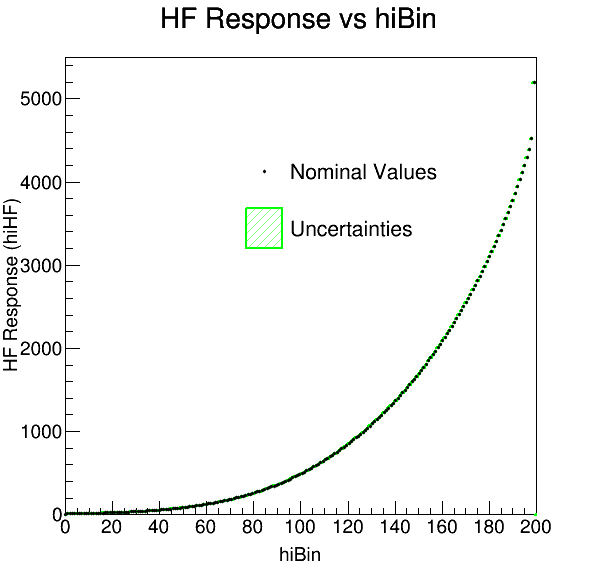
\includegraphics[width= 0.48\textwidth]{Figures/Chapter4/hiHFvsCent.png}
\caption{The nominal (black) and uncertainties band (green) hiHF vs hiBin for CMS 2018 PbPb dataset are shown above.}
\label{hiHFvsCent}
\end{center}
\end{figure}


We can compute the percent deviation nom of final results to estimate systematics due to uncertainties of centrality. 


\subsection{$\langle N_{part} \rangle$, $\langle N_{coll} \rangle$, $\langle T_{AA} \rangle$ vs Centrality}

As we discussed in the Glauber Model \cite{CentPlot,Glauber} section 1.5.7, the number of participant nucleons $N_{part}$, the number of binary nucleon-nucleon collisions, and nuclear over lapping function $T_{AA}$ are all functions of the event centrality. The CMS Global Observable group has computed the average $N_{part} $, $N_{coll} $, $T_{AA}$ and their uncertainties  for different centrality bins based on the Glauber Model. The selected results are shown Table \ref{GOvsCent} below


\begin{table}[h]
\begin{center}
\caption{Summary table of the total number of MB events vs centrality is shown below. The uncertainties are represented in terms of percentage in the parenthesis.}
\vspace{1em}
\label{GOvsCent}
  \begin{tabular}{ |c | c| c| c|}
    \hline 
Centrality &  $\langle N_{part} \rangle$ &$\langle N_{coll} \rangle$  & $\langle T_{AA} \rangle$  \\
     \hline
         \hline
0-30\% &  269.1 (0.39\%)  &  1042 (2.0\%) &	15.42 (2.0\%)   \\
30-90\% & 54.45 (1.5\%)   & 115.2 (3.6\%)  &   1.704 (3.6\%)  \\
0-90\% & 126.0 (0.67\%)   &  424.1(2.2\%)  &    6.274 (2.2\%)  \\
     \hline
    \hline
\end{tabular}
\end{center}
\end{table}

The global observables $N_{MB}$, $N_{part}$, $N_{coll}$, and $T_{AA}$ will be used inputs for our B-meson analysis. 

\iffalse

\subsection{Number of Participant Nucleons}

\subsection{Number of Binary Collisions}


\fi

\subsection{Event Multiplicity}

Aside from $N_{MB}$, $N_{part}$, $N_{coll}$, and $T_{AA}$, event multiplicity is also an event observable. We count the number of tracks in each event with some track quality selections and use it to interpret the event multiplicity, which characterizes the event activity. The following is the selection criteria for 

Nevertheless, the event multiplicity is not used in PbPb analysis. It will be used in $pp$ analysis to study the $B^0_s/B^+$ ratio as a function of event multiplicity in $pp$ collisions.

%\section{Monte Carlo Simulations} 

%The Monte Carlo (MC) simulation on the B meson decay is essential to the analysis. It will plays an important role in both the signal extraction and efficiency correction.

%\subsection{PYTHIA}

%\subsection{Hydjet Embedding}

%\subsection{EvtGen Package}

%\subsection{MC reweighing}

\section{B meson Reconstruction} 

Now we look into each events of the PbPb dimuon dataset. It turns out that there is no PU in any event. Therefore, only one primary vertex for each event. We can then reconstruct the B meson candidates according to the final state muons and kaons tracks. In CMS, a dedicated software named ``\textit{Bfinder}'' is developed to perform B-meson reconstruction. Figure \ref{BsRECOWF} and \ref{BPRECOWF} show the workflow to fully reconstruct \textit{Bfinder} for $B^0_s$ and $B^+$ respectfully.


\begin{figure}[h]
\begin{center}
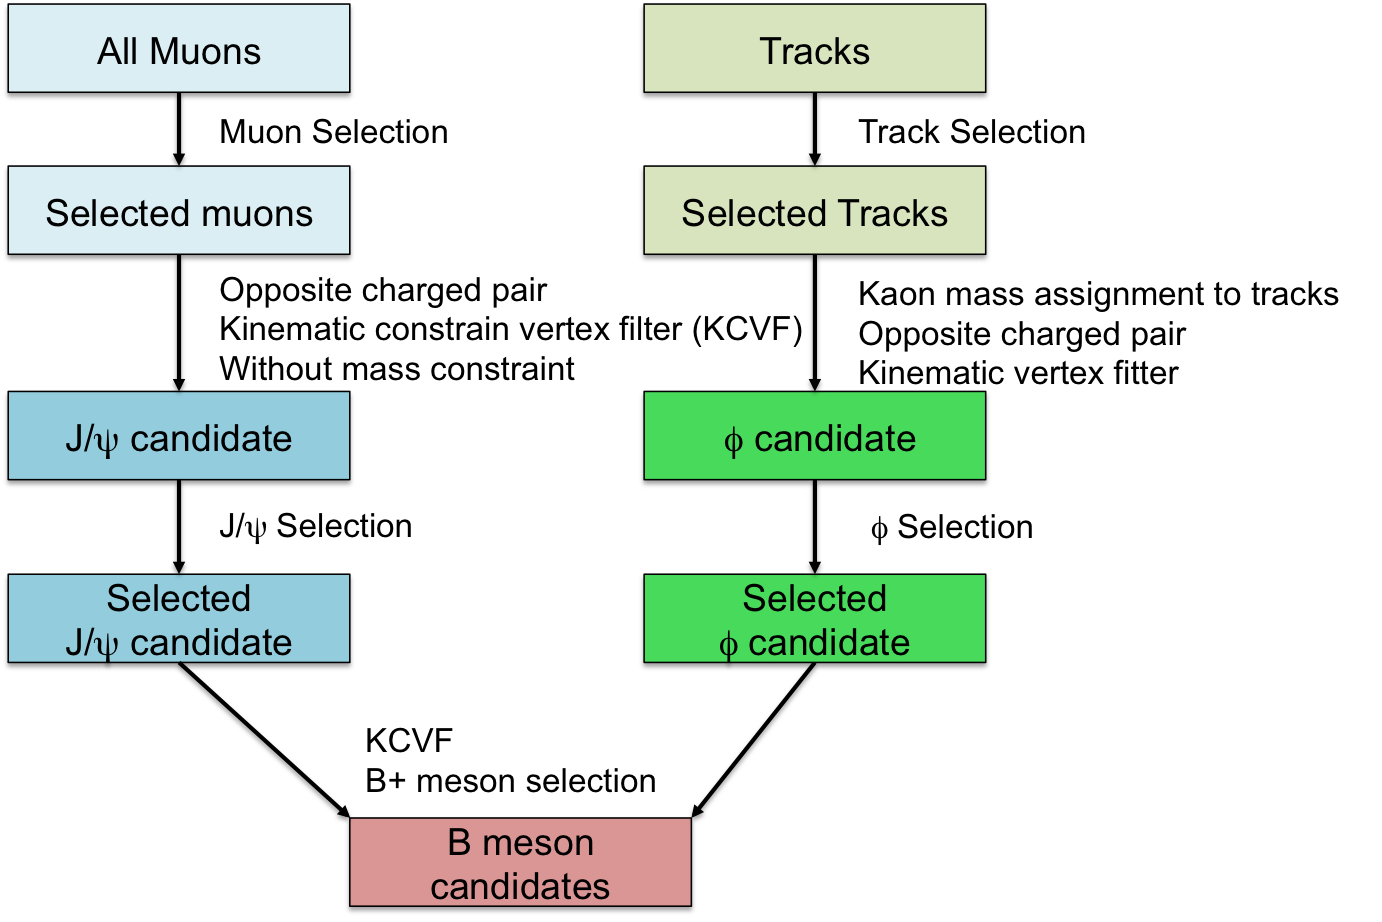
\includegraphics[width= 0.98\textwidth]{Figures/Chapter4/BsmesonWorkflow.png}
\caption{The schematic block diagram of the full reconstruction workflows for $B^0_s$ via the decay channel of $B_s^0 \rightarrow J/\psi \phi \rightarrow \mu^+\mu^- K^+K^-$ in the \textit{Bfinder} is shown above.}
\label{BsRECOWF}
\end{center}
\end{figure}

\begin{figure}[h]
\begin{center}
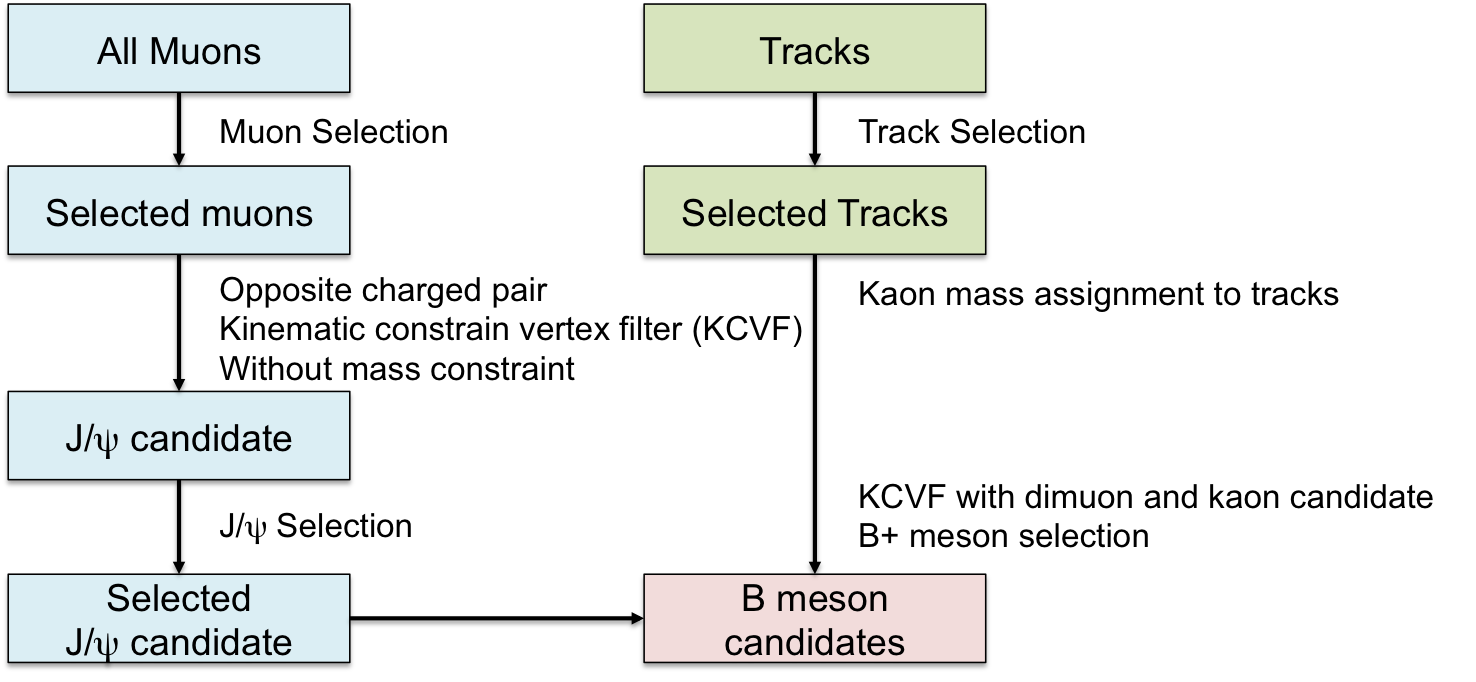
\includegraphics[width= 0.98\textwidth]{Figures/Chapter4/BPmesonWorkflow.png}
\caption{The schematic block diagram of the full reconstruction workflows for $B^+$ via the decay channel of $B^+ \rightarrow J/\psi K^+ \rightarrow \mu^+\mu^- K^+$ in the \textit{Bfinder} is shown above.}
\label{BPRECOWF}
\end{center}
\end{figure}

Here, we should note that since we do not have hadronic PID for the kaons, we assume the track to be kaons and assume the charged kaon PDG mass to the tracks \cite{PDG} to the tracks.

%\subsection{Decay Channels}

\subsection{Event Selections}

To ensure the quality of inelastic hadronic collisions events for B-meson reconstruct, we apply the follow selections


\begin{itemize}
\item At least one reconstructed primary interaction vertex, formed by two or more tracks
\item The longitudinal distance from the center of the nominal interaction region of less than 15 cm along the beam axis: $|$PV$_{z}$$| < $ 15
\item Compatible shapes of the clusters in the pixel detector with those expected from particles produced by a PbPb collision
\item At least two towers in each of the HF detectors with energy deposits of more than 4GeV per tower  
\end{itemize}

\subsection{Track Selections}



\subsection{Muon Selections}


\subsection{Performance}

\section{MC-Data Comparison}

Ideally, if the simulation is impeccable, the RECO distribution in the MC should match perfectly with data. Nevertheless, there is always limitation in the MC simulation because the incorrect model of physics processes in the generation side or poor model of detector conditions the in the reconstruction side. The discrepancy should be corrected  


\section{Background Studies} 




\section{Cut Optimization} 

\subsection{Topological Variables}

\subsection{Multivariate Analysis}

\subsection{Machine Learning Techniques}

\subsection{Training Performance}

\subsection{Working Point Determination}


\section{Signal Extraction} 

\subsection{B-meson Invariant Mass Distributions}

\subsection{Fitting Models}

\subsection{Raw Yield Extraction}

\subsection{Signal Significance Estimation}


\section{Acceptance and Efficiency Correction} 

\subsection{Analysis Challenges}

\subsection{Fiducial Measurement}

\subsection{Fine 2D Efficiency Map}

\subsection{Data-Drive Efficiency Correction}

\subsection{Tag \& Probe Techniques}

\subsection{Nominal Results}

\section{Cross Section Results} 

\section{Validation Tests} 

\subsection{Mass Scraping Test}

\subsection{Raw Yield Closure}

\subsection{Efficiency Closure}

\subsection{sPlot Closure}


\section{Statistical Uncertainties Determination} 

\subsection{Data Bootstrapping}

\subsection{Statistical Uncertainties Interpretation}

\section{Systematic Uncertainties Estimation} 

\subsection{Global Observables}

\subsection{Branching Ratios}

\subsection{Tracking Efficiency}

\subsection{Muon Efficiency}

\subsection{Selection Efficiency}

\subsection{Signal Extraction}

\subsection{Summary}

\section{Final Results} 

\subsection{$B^0_s$ and $B^{+}$ Cross Section}

\subsection{$B^0_s/B^{+}$ Ratio}

\subsection{$B^0_s$ and $B^{+}$ Nuclear Modification Factor}

